% Section 7.2 -- E2: initialisation strategies (P2)
% Numbers from results/E2/E2_init.csv (p = 6, means over 10 instances per n).
% This file also holds the E6 figure, so E2 and E6 share one figure page.

\subsection{E2: Initialisation strategies}
\label{sec:e2}

E2 compares four starting points at $p = 6$ on the same ten instances per size $n = 10$--$16$: INTERP, the best of five random starts, and angles transferred from the $n = 8$ instances of E1, with and without optimisation.

\begin{figure}[p]
  \centering
  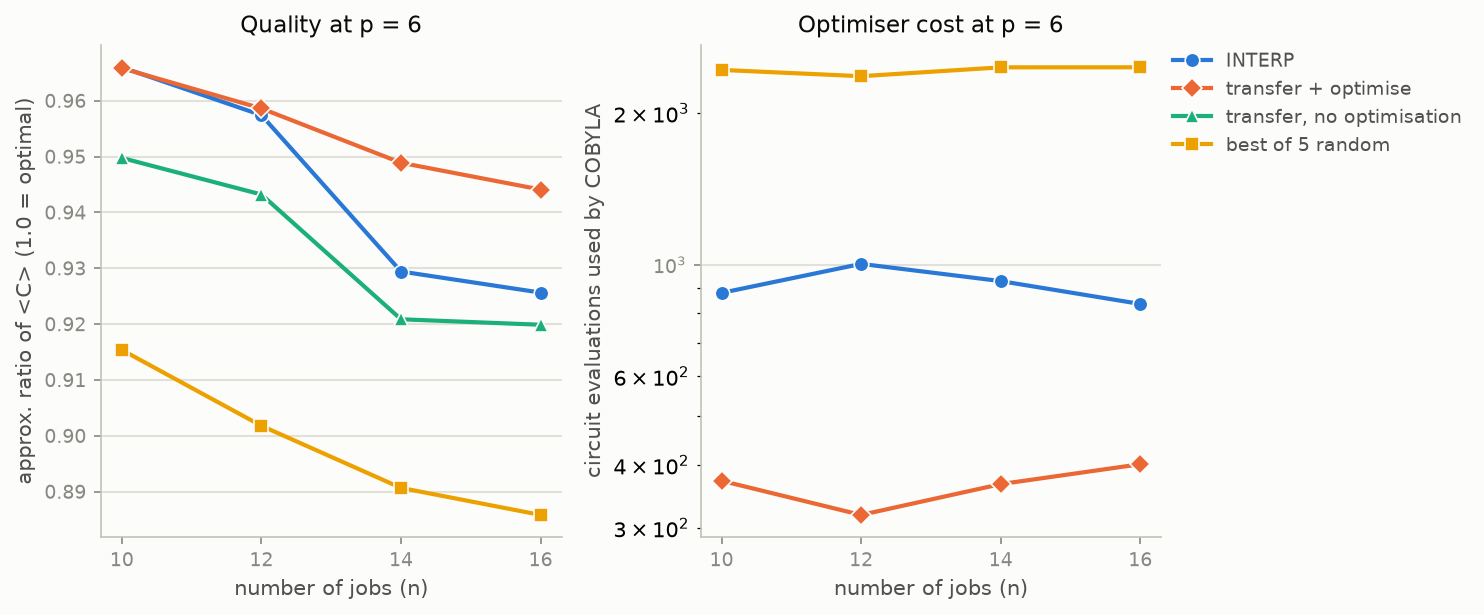
\includegraphics[width=\linewidth]{E2_init.png}
  \caption{E2 at $p = 6$. Left: approximation ratio of the mean cost. Right: circuit evaluations used by COBYLA (log scale); for INTERP this counts the whole chain $p = 1, \dots, 6$.}
  \label{fig:e2}
  \vspace{18pt}
  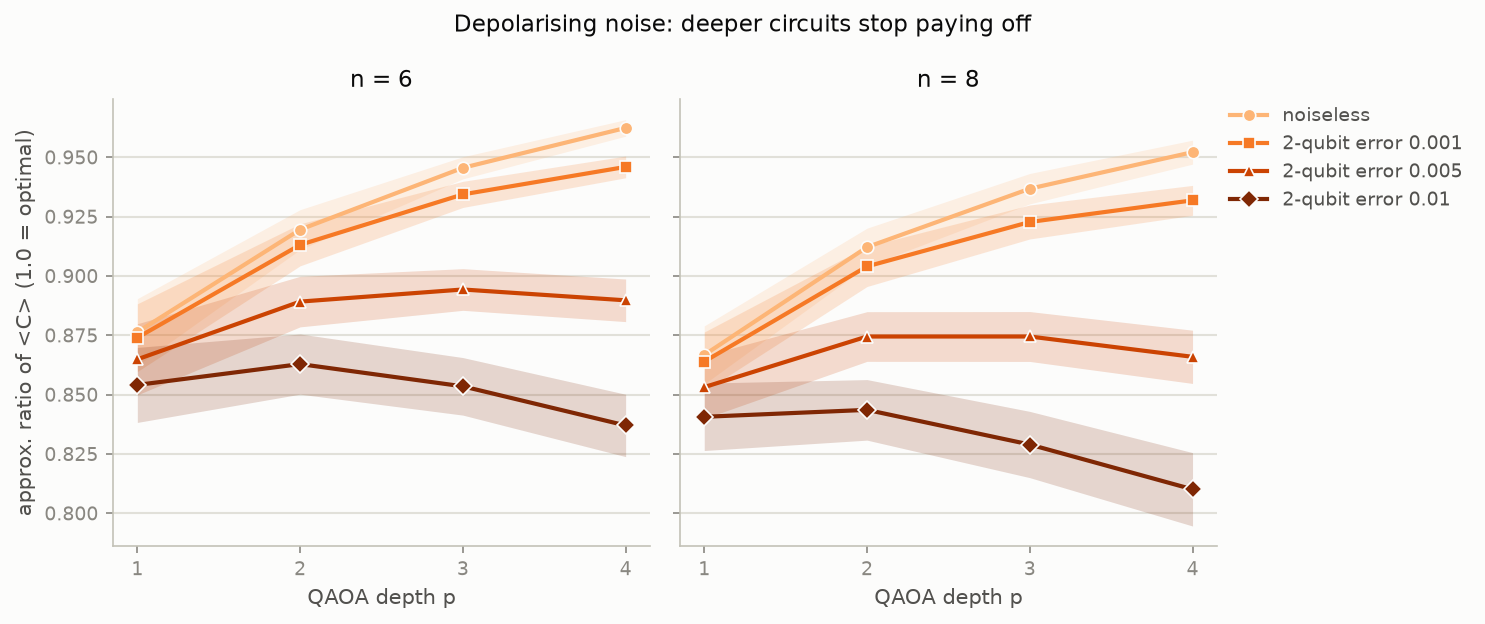
\includegraphics[width=\linewidth]{E6_noise.png}
  \caption{E6. Approximation ratio of the mean cost against depth for each two-qubit error rate, at $n = 6$ (left) and $n = 8$ (right).}
  \label{fig:e6}
\end{figure}

Transfer followed by optimisation gives the best quality at every size, with a mean ratio of $0.954$, against $0.945$ for INTERP, $0.933$ for transfer without optimisation and $0.898$ for random starts (Fig.~\ref{fig:e2}).
It is also cheap: about 360 evaluations, 40\,\% of INTERP's 910 over its full chain and 15\,\% of the 2{,}430 used by random starts.
The gap to INTERP comes from only two instances: the two on which INTERP is stuck in E1, where transfer reaches $0.961$ and $0.915$; without them both average $0.955$.
Even with no optimisation, transferred angles reach $0.933$, so good angles are similar across instances and sizes, which E5 exploits.
